\documentclass{scrartcl}
\usepackage[utf8]{inputenc}
\usepackage[T1]{fontenc}
\usepackage{verbatim}
\usepackage{enumitem}
\usepackage{graphicx}
\usepackage[ngerman]{babel}
\usepackage{hyperref}
\usepackage{xcolor}
\usepackage{pdfpages}
\setlength{\parindent}{0em} 
\setcounter{secnumdepth}{4}
\setcounter{tocdepth}{4} 
\hypersetup{
    colorlinks,
    linkcolor={blue!65!black},
    citecolor={blue!50!black},
    urlcolor={blue!80!black}
}
\title{goApp Qualitätssicherung}
\author{Jörn Kussmaul, Katharina Riesterer, Julian Neubert,\\ Jonas Walter, Tobias Ohlsson, Eva-Maria Neumann}
\begin{document}
	\maketitle
	\newpage
	\tableofcontents
	\newpage

\section{Einleitung}
In der Phase der Qualitätssicherung ging es uns darum Fehler der goApp zu finden und zu beheben.
Allen voran kann die App jetzt den auf dem Server berechneten Gruppenmittelpunkt bei Terminen anzeigen.
\newline
Ebenfalls haben wir weitere Unit-Tests zur Erhöhung der Code-Überdeckung und zur Überprüfung von Randfällen implementiert um möglichst viele Fehler zu finden und eine hervorragende user experience zu bieten.
\newline
Ob uns dies gelungen ist haben wir versucht über das verbreiten der App unter Beta Usern herauszufinden.
Hiervon versprachen wir uns konstruktive Kritik, insbesondere an der GUI um diese für den User noch intuitiver zu gestalten. 
Ansonsten haben wir unser Projekt durch Werkzeuge wie Lint, ein Tool zur statischen Analyse von Code, und Monkey Test überprüft um die Code Qualität noch weiter zu steigern.

Auf weitere Änderungen sowohl am Design als auch der Funktionalität der goApp gehen wir im folgendem Dokument ein.

\newpage
\section{Server}
\subsection{SonarLint}
SonarLint ist ein Programm zur statischen Code-Analyse der Quelltexte von Computerprogrammen. Mit SonarLint überprüfen wir unseren Servercode um mögliche Bugs zu finden und unsere Codequalität zu steigern.
Dadurch haben wir unter anderem das Fehlen einer break Anweisung gefunden.

\subsection{Änderungen}
Während der Qualitätssicherung bemerkten wir durch unsere Tests noch einige kleine Fehler im Code. Diese wurden behoben und sind im folgenden zusammen mit kleineren Optimierungen aufgeführt.
\subsubsection{Algorithmus}
Beim Testen ist uns aufgefallen, dass die Clusterberechnung bei verschiedenen Größenordnungen an Abständen der Mitglieder schlechte Ergebnisse  liefert, da der Radius, der festlegt wann man zusammen in ein Cluster gezählt wird, fest und nicht dynamisch ist. Aus diesem Grund haben wir uns nun dazu entschieden eine weitere, speziell auf den Clusteralgorithmus DBSCAN festgelegte, Methode anzubieten, die verschiedene Radien bei der Berechnung benutzt. Die Methode basiert auf der Rahmenbedingung, dass mindestens 3 von 4 Mitglieder bei der Berechnung der der Mittelpunkte berücksichtigt werden sollen, was äquivalent zu der Aussage ist, dass mindestens 3 von 4 Mitglieder sich nach der Clusterberechung in Cluster mit mehr als einer Person befinden. Wir suchen also nach den kleinsten Cluster, so dass die Rahmenbedingung erfüllt ist. Diese Suche wurde mit Hilfe einer Schleife implementiert, wobei bei jedem Schleifendurchlauf der Parameter, der angibt welchen Abstand Clustermitglieder zueinander haben dürfen, verdoppelt wird. Um unseren Server vor vor ewigen Laufzeiten zu schützen haben wir zusätzlich eine maximale Schleifendurchlaufszahl von 12 festgelegt, was einem Radius von über 200 Kilometer entspricht und somit für jede sinnvolle Nutzung unserer App ausreicht.
\subsubsection{Datenbank}
Es gab einen Fehler im Zusammenhang mit dem LocationDeletionTimer und dem EventDeletionTimer, welche sich um das Löschen alter Events und alter Locations kümmern.
\begin{itemize} 
\item Fehlersymptom:
Mehrere der Timer liefen gleichzeitig. Und es gab Timer mit zum Teil veralteten Einstellungen (Dauer bis zum löschen).
\item Fehlergrund:
Alte Timer wurden niemals beendet und liefen auch nach erneutem Hochladen weiter. Dadurch kam bei jedem hochladen auf den Server ein weiterer Timer hinzu.
\item Fehlerbehebung:
Wir haben eine neue Klasse die das Interface ServletContextListener implementiert erstellt. Das Interface deklariert die zwei Methoden contextInitialized und contextDestroyed. Diese werden aufgerufen, wenn die Web-App gestartet bzw. beendet wird.
Anstatt beim erstellen der SessionFactory werden die zwei Timer deshalb jetzt in dieser Klasse gestartet und dort auch wieder beendet.
\end{itemize}
Zudem zeigten neue Assertions in den Tests, dass die Parameter nicht immer auf null überprüft wurden. Zum Beispiel in der Klasse GroupManagement bei der Methode public boolean update(Group chGroup). An diesen stellen wurden die entsprechenden Überprüfungen ergänzt.\newline

Zusätzlich zu dem Beheben von Fehlern wurden noch folgende Sachen verändert:
\begin{itemize} 
\item Der bei der Datenbank voreingestellte Connection Pool, welcher nur zum Testen verwendet werden sollte, wurde durch den c3p0 Pool ersetzt.
\item Die Termine werden nun immer aufsteigend nach Datum sortiert zurückgegeben, damit sie auf dem Client nicht immer in einer anderen Reihenfolge erscheinen und man die aktuellsten Termine als erstes sieht.
\item Gruppen und User werden nun immer aufsteigend nach dem Namen zurückgegeben.
\end{itemize}
\subsubsection{Servlet}

\paragraph{RequestServlet}
\begin{itemize} 
\item Fehlersymptom: Es tritt eine NullPointerException in der Methode create auf.
\item Fehlergrund: Der Nutzer ist in keiner Gruppe Mitglied oder hat noch keine Anfrage gesendet.
\item Fehlerbehebung: Es wird geprüft ob Gruppen bzw. Anfragen existieren und falls nicht entsprechend reagiert.
\end{itemize}
\paragraph{UserServlet}
\begin{itemize} 
\item Fehlersymptom: Es tritt in der Methode changeName eine NullPointerException auf.
\item Fehlergrund: Wenn ein Nutzer in der Datenbank nicht gefunden wird, gibt diese null zurück. Dies wurde nicht geprüft.
\item Fehlerbehebung: Vor der weiteren Ausführung wird die Antwort der Datenbank geprüft.
\end{itemize}
\paragraph{EventServlet}
\begin{itemize} 
\item Fehlersymptom: Es wurde trotz eines Fehlers, der Fehlercode für OK zurück gegeben.
\item Fehlergrund: Die Rückgabe des Fehlercodes an Stelle, wo der Fehler gefunden wurde hat gefehlt.
\item Fehlerbehebung: Der Fehlercode wird jetzt zurück gegeben.
\end{itemize}
\newpage


\subsection{Tests}
Zu den Unit-Tests aus der Implementierungsphase sind weitere Tests dazugekommen um die Abdeckung zu erhöhen, sowie Randfälle zu testen.
\subsubsection{Algorithmus}
Wie oben beschrieben stellen wir eine weitere Methode zur Berechnung der Cluster und deren Mittelpunkte zur Verfügung. Diese Methode wurde nun auch ausführlich mit Hilfe von Unittests getestet. Dabei wurden wieder verschiedenen Testpunkte initialisiert und die Verbindung zur Datenbank mit Mockito gemockt, um den Algorithmus separat zu testen.
\subsubsection{Datenbank}
Bei den Tests für die Datenbank kamen nur zwei neue Testmethoden hinzu.
Es wurden aber die bestehenden um Assertions ergänzt, welche Randfälle wie eine falsche id oder einen Parameter bei dem null übergeben wird überprüfen.
\paragraph{EventManagement}
\subparagraph{public void testDeleteOldEvents()}
Der Test überprüft, ob das löschen alter Events aus der Datenbank funktioniert.
\paragraph{LocationDeletionTimer}
\subparagraph{public void testTimerStarter()}
Der Test stellt sicher, dass die Methoden contextInitialized und contextDestroyed des ServletContextListeners den LocationDeletionTimer korrekt starten und beenden.


\subsubsection{Servlet}

\paragraph{RequestServlet}
\subparagraph{public void testCreateUserIsMember()}
Dieser Test überprüft das Verhalten des Servlets, wenn der Nutzer schon Mitglied in der angefragten Gruppe ist. Erwartet wird ein Interact Fehler.
\subparagraph{public void testCreateUserHasRequest()}
Dieser Test überprüft das Verhalten des Servlets, wenn der Nutzer schon eine offene Anfrage an die Gruppe hat. Erwartet wird ein Interact Fehler.
\subparagraph{public void testCreateUserLimitReached()}
Es wird überprüft ob ein USR\_LIMIT Fehler gesendet wird, wenn der Nutzer schon in zu vielen Gruppen Mitglied ist.
\subparagraph{public void testCreateGroupLimitReached()}
Es wird überprüft ob ein GRP\_LIMIT Fehler gesendet wird, wenn die Gruppe ihr Mitglieder Limit schon erreicht hat.
\subparagraph{public void testCreateDatabaseAddFalse()}
Dieser Test überprüft das Verhalten, wenn die Datenbank beim Hinzufügen der Gruppe und des Nutzers zur Datenbank false zurück gibt. Erwartet wird ein DB\_ERROR.
\subparagraph{public void testCreateDatabaseReqByGroupNull()}
Es soll kein Fehler auftreten, wenn die Datenbank bei den Anfragen zu einer bestimmten Gruppe null zurück gibt, weil momentan keine existieren.
\subparagraph{public void testCreateDatabaseReqByUserNull()}
Es soll kein Fehler auftreten, wenn die Datenbank bei den Anfragen zu einem bestimmten Nutzer null zurück gibt, weil momentan keine existieren.
\subparagraph{public void testCreateDatabaseGetUserNull()}
Es soll ein Fehler auftreten, wenn der Nutzer nicht in der Datenbank existiert.
\subparagraph{public void testCreateDatabaseGetGroupsNull() }
Es soll ein Fehler auftreten, wenn die Gruppe nicht in der Datenbank existiert.
\subparagraph{public void testCreateWOutJSON()}
Die Methode create wird ohne alle erforderlichen JSON Parameter aufgerufen. Es soll ein READ\_JSON Fehler zurückgegeben werden.
\subparagraph{public void testAcceptDatabaseAddFalse()}
Es soll ein DB\_ERROR entstehen, wenn die Datenbank beim Hinzufügen einer Gruppen/Nutzer Kombination false zurückgibt.
\subparagraph{public void testRejectDatabaseDeleteFalse()}
Es soll ein DB\_ERROR entstehen, wenn die Datenbank beim Löschen einer Gruppen/Nutzer Kombination false zurückgibt.
\subparagraph{public void testRejectDatabaseRequestNull()}
Es soll ein DB\_ERROR entstehen, wenn die Datenbank keine Anfrage vom Nutzer an die Gruppe findet.
\subparagraph{public void testAcceptWOutJSON()}
Die Methode accept wird ohne alle erforderlichen JSON Parameter aufgerufen. Es soll ein READ\_JSON Fehler zurückgegeben werden.
\subparagraph{public void testRejectWOutJSON() }
Die Methode reject wird ohne alle erforderlichen JSON Parameter aufgerufen. Es soll ein READ\_JSON Fehler zurückgegeben werden.
\subparagraph{public void testMethodNotExisting()}
Wenn eine Methode augerufen wird, die in dem Servlet nicht existiert, soll ein METH\_ERROR zurück gegeben werden.
\subparagraph{public void testEmptyJSON()}
Wenn ein leerer JSON String übergeben wird, soll der Fehler READ\_JSON entstehen.

\paragraph{RequestSearchServlet}
\subparagraph{public void testGetRequestsByUserDatabaseNull()}
Wenn keine Anfragen von einem bestimmten Nutzer existieren gibt die Datenbank null zurück. Das Ergebnis der Methode soll ein Fehlercode EMPTY\_LIST sein.
\subparagraph{public void testGetRequestsByUserWOutJSON()}
Die Methode getRequestsByUser wird ohne alle erforderlichen JSON Parameter aufgerufen. Es soll ein READ\_JSON Fehler zurückgegeben werden.
\subparagraph{public void testGetRequestsByGroupDatabaseNull()}
Wenn keine Anfragen an eine bestimmte Gruppe existieren gibt die Datenbank null zurück. Das Ergebnis der Methode soll ein Fehlercode EMPTY\_LIST sein.
\subparagraph{public void testGetRequestsByGroupWOutJSON()}
Die Methode getRequestsByGroup wird ohne alle erforderlichen JSON Parameter aufgerufen. Es soll ein READ\_JSON Fehler zurückgegeben werden.
\subparagraph{public void testMethodNotExisting()}
Wenn eine Methode aufgerufen wird, die in dem Servlet nicht existiert, soll ein METH\_ERROR zurück gegeben werden.
\subparagraph{public void testEmptyJSON()}
Wenn ein leerer JSON String übergeben wird, soll der Fehler READ\_JSON entstehen.

\paragraph{UserServlet}
\subparagraph{public void testMethodNotExisting()} 
Wenn eine Methode aufgerufen wird, die in dem Servlet nicht existiert, soll ein METH\_ERROR zurück gegeben werden.
\subparagraph{public void testEmptyJSON()}
Wenn ein leerer JSON String übergeben wird, soll der Fehler READ\_JSON entstehen.
\subparagraph{public void testChangeNameDatabseNullGetUser()}
Es soll ein DB\_ERROR zurückgegeben werden, wenn die Datenbank beim Aufruf der Methode getUser null zurückgibt (d.h. der Nutzer wurde nicht gefunden).
\subparagraph{public void testChangeNameDatabseFalseUpdate()}
Es soll ein DB\_ERROR zurückgegeben werden, wenn die Datenbank beim Aufruf der Methode update vom User false zurückgibt.
\subparagraph{public void testChangeNameWOutJSON()}
Die Methode changeName wird ohne alle erforderlichen JSON Parameter aufgerufen. Es soll ein READ\_JSON Fehler zurückgegeben werden.

\paragraph{EventServlet}
\subparagraph{public void testMethodNotExisting()}
Wenn eine Methode aufgerufen wird, die in dem Servlet nicht existiert, soll ein METH\_ERROR zurück gegeben werden.
\subparagraph{public void testEmptyJSON()}
Wenn ein leerer JSON String übergeben wird, soll der Fehler READ\_JSON entstehen.
\subparagraph{public void testCreateDatabaseNull()}
Es wird ein DB\_ERROR erwartet, wenn die die Datenbank das Event nicht angelegen konnte und deswegen null zurückgibt.
\subparagraph{public void testCreateWOutJSON()}
Die Methode create wird ohne alle erforderlichen JSON Parameter aufgerufen. Es soll ein READ\_JSON Fehler zurückgegeben werden.
\subparagraph{public void testGetParticipatesDatabaseNull()}
Es wird ein EMPTY\_LIST Fehler erwartet, wenn die die Datenbank keiner Nutzer beim event mit der übergebenen EventID gefunden hat und deswegen null zurückgibt.
\subparagraph{public void testGetParticipatesWOutJSON()}
Die Methode getParticipates wird ohne alle erforderlichen JSON Parameter aufgerufen. Es soll ein READ\_JSON Fehler zurückgegeben werden.
\subparagraph{public void testChangeWOutEventId()}
Wenn der JSONParameter EventId bei der Methode change fehlt, soll der Fehler READ\_JSON entstehen.
\subparagraph{public void testChangeDatabaseWrong()}
 Wenn die Datenbank das Event nicht updaten konnte und deswegen false zurück gibt, soll ein DB\_ERROR entstehen.
 
\paragraph{ParticipateServlet}
\subparagraph{public void testSetStatsuWOutJSON()}


\paragraph{LocationServlet}
\subparagraph{public void missingMethod()}
Das LocationServlet wird ohne den Parameter für die Methode aufgerufen, so dass der Fehlercode READ\_JSON zurückgegeben wird.
\subparagraph{public void invalidMethod()}
Es wird versucht eine Methode aufzurufen, die in diesem Servlet nicht existiert. Der METH\_ERROR Fehlercode soll an den Client gesendet werden.
\subparagraph{public void missingParameter()}
Die Methode wird korrekt aufgerufen, jedoch fehlt ein Parameter zur korrekten Ausführung. Der METH\_ERROR Fehler wird zurückgegeben.
\subparagraph{public void getClusterError()}
Beim Abfragen des Events tritt ein Fehler in der Datenbank auf und das Servlet gibt den DB\_ERROR zurück.

\paragraph{GroupServlet}
\subparagraph{public void invalidMethod()}
Es wird versucht eine Methode aufzurufen, die in diesem Servlet nicht existiert. Der METH\_ERROR Fehlercode soll an den Client gesendet werden.
\subparagraph{public void missingMethod()}
Das GroupSearchServlet wird ohne den Parameter für die Methode aufgerufen, so dass der Fehlercode READ\_JSON zurückgegeben wird.
\subparagraph{public void createMissingParameter()}
Die Methode wird korrekt aufgerufen, jedoch fehlt ein Parameter zur korrekten Ausführung. Der METH\_ERROR Fehler wird zurückgegeben.
\subparagraph{public void createDatabaseError()}
Es wird versucht eine neue Gruppe zu erstellen, jedoch tritt beim erstellen des Datenbankeintrags ein Fehler auf und es wird null zurückgegeben. Das Servlet sendet den DB\_ERROR Fehlercode an den Client.
\subparagraph{public void deleteMissingParameter()}
Die Methode wird korrekt aufgerufen, jedoch fehlt ein Parameter zur korrekten Ausführung. Der METH\_ERROR Fehler wird zurückgegeben.
\subparagraph{public void deleteDatabaseError()}
Es wird versucht eine Gruppe zu löschen, jedoch tritt beim entfernen des Datenbankeintrags ein Fehler auf und es wird null zurückgegeben. Das Servlet sendet den DB\_ERROR Fehlercode an den Client.
\subparagraph{public void setNameMissingParameter()}
Die Methode wird korrekt aufgerufen, jedoch fehlt ein Parameter zur korrekten Ausführung. Der METH\_ERROR Fehler wird zurückgegeben.
\subparagraph{public void setNameDatabaseError()}
Es wird versucht den Namen einer Gruppe zu ändern, jedoch tritt beim ändern des Datenbankeintrags ein Fehler auf und es wird null zurückgegeben. Das Servlet sendet den DB\_ERROR Fehlercode an den Client.
\subparagraph{public void deleteMemberMissingParameter()}
Die Methode wird korrekt aufgerufen, jedoch fehlt ein Parameter zur korrekten Ausführung. Der METH\_ERROR Fehler wird zurückgegeben.
\subparagraph{public void deleteMemberDatabaseError()}
Es wird versucht ein Mitglied aus einer Gruppe zu entfernen, jedoch tritt beim entfernen des Datenbankeintrags ein Fehler auf und es wird null zurückgegeben. Das Servlet sendet den DB\_ERROR Fehlercode an den Client.
\subparagraph{public void getEventsMissingParameter()}
Die Methode wird korrekt aufgerufen, jedoch fehlt ein Parameter zur korrekten Ausführung. Der METH\_ERROR Fehler wird zurückgegeben.
\subparagraph{public void getEventsDatabaseParticipantsError()}
Es wird versucht die Liste von Events in einer Gruppe abzufragen, jedoch tritt beim abrufen des Datenbankeintrags ein Fehler auf und es wird null zurückgegeben. Das Servlet sendet den DB\_ERROR Fehlercode an den Client.
\subparagraph{public void getEventsDatabaseStartedError()}
Es wird versucht die Liste von Events in einer Gruppe abzufragen, jedoch tritt beim abrufen des Datenbankeintrags ein Fehler auf und es wird null zurückgegeben. Das Servlet sendet den DB\_ERROR Fehlercode an den Client.
\subparagraph{public void getEventsDatabaseInvitedError()}
Es wird versucht die Liste von Events in einer Gruppe abzufragen, jedoch tritt beim abrufen des Datenbankeintrags ein Fehler auf und es wird null zurückgegeben. Das Servlet sendet den DB\_ERROR Fehlercode an den Client.
\subparagraph{public void getMembersMissingParameter()}
Die Methode wird korrekt aufgerufen, jedoch fehlt ein Parameter zur korrekten Ausführung. Der METH\_ERROR Fehler wird zurückgegeben.
\subparagraph{public void getMembersDatabaseError()}
Es wird versucht die Liste von Mitgliedern der gegebenen Gruppe abzufragen, jedoch tritt beim abrufen des Datenbankeintrags ein Fehler auf und es wird null zurückgegeben. Das Servlet sendet den DB\_ERROR Fehlercode an den Client.
\subparagraph{public void setFounderMissingParameter()}
Die Methode wird korrekt aufgerufen, jedoch fehlt ein Parameter zur korrekten Ausführung. Der METH\_ERROR Fehler wird zurückgegeben.
\subparagraph{public void setFoundergetUserDatabaseError()}
Es wird versucht den Gründer einer Gruppe zu ändern, jedoch tritt beim abfragen des Users des Gründers aus der Datenbankeintrags ein Fehler auf und es wird null zurückgegeben. Das Servlet sendet den DB\_ERROR Fehlercode an den Client.
\subparagraph{public void setFounderDatabaseError()}
Es wird versucht den Namen einer Gruppe zu ändern, jedoch tritt beim ändern des Datenbankeintrags ein Fehler auf und es wird null zurückgegeben. Das Servlet sendet den DB\_ERROR Fehlercode an den Client.

\paragraph{GroupSearchServlet}
\subparagraph{public void missingMemberSearch()}
Es wird eine Anfrage gesendet, eine Gruppe mit dem gegebenen Mitglied zu suchen, die UserID des Mitglieds wird jedoch nicht als Parameter übergeben. Das Servlet antwortet mit einem READ\_JSON Fehlercode.
\subparagraph{public void groupNonExistentMemberSearch()}
Eine Suchanfrage wird an das Servlet gesendet, in der nach einer Gruppe mit einem gegeben Mitglied gesucht wird, jedoch existiert keine Gruppe mit dem Mitglied in der Datenbank. Die Datenbank gibt null zurück und der Client erhält einen DB\_ERROR.
\subparagraph{public void missingNameSearch()}
Es wird eine Anfrage gesendet, eine Gruppe mit dem gegebenen Namen zu suchen, der Name wird jedoch nicht als Parameter übergeben. Das Servlet antwortet mit einem READ\_JSON Fehlercode.
\subparagraph{public void groupNonExistentNameSearch()}
Eine Suchanfrage wird an das Servlet gesendet, in der nach einer Gruppe mit dem Namen gesucht wird, jedoch existiert keine Gruppe mit dem Namen in der Datenbank. Die Datenbank gibt null zurück und der Client erhält einen DB\_ERROR.
\subparagraph{public void invalidMethod()}
Es wird versucht eine Methode aufzurufen, die in diesem Servlet nicht existiert. Der METH\_ERROR Fehlercode soll an den Client gesendet werden.
\subparagraph{public void missingMethod()}
Das GroupSearchServlet wird ohne den Parameter für die Methode aufgerufen, so dass der Fehlercode READ\_JSON zurückgegeben wird.

\newpage
\subsubsection{Abdeckung}
\paragraph{EclEmma}
EclEmma ist ein Plugin für Eclipse, welches die Testabdeckung misst. Dabei wird bei der Ausführung einer Anwendung festgestellt, welche Klassen, Methoden, Blöcke und Zeilen Code ausgeführt wurden. 
Mit diesem Tool haben wir die Abdeckung durch unsere Tests geprüft.
\paragraph{}
Die Testabdeckung für den Server beträgt 90,8\%.
Nach der Implementierungsphase mit Tests zur Funktionalität betrug die Abdeckung 76,5\%.
%\begin{figure}[h]
%	\centering
%	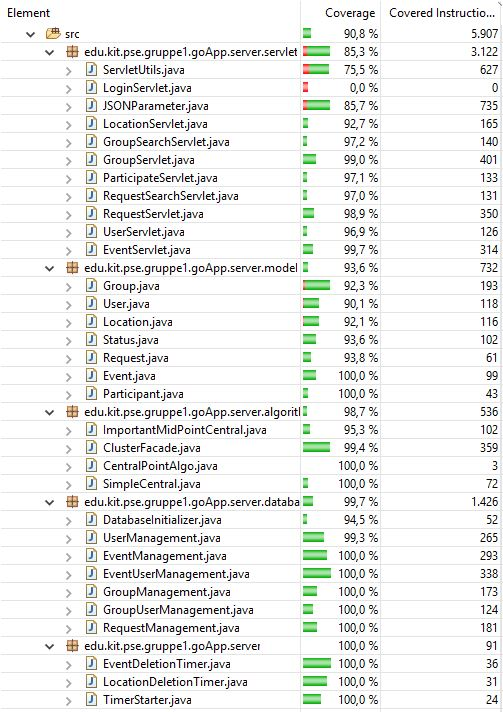
\includegraphics[width=0.7\textwidth]{Codeabdeckung.jpg}
%	\caption{Codeabdeckung}
%\end{figure}

\begin{center}
	\makebox [0pt]{	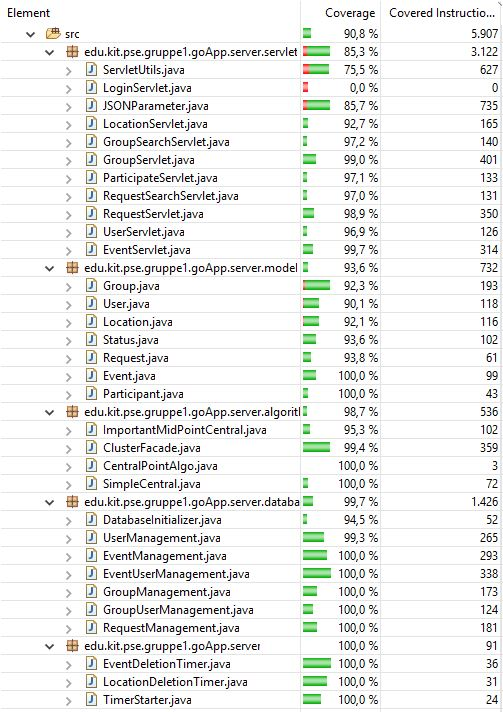
\includegraphics[height=0.79\textheight]{Codeabdeckung.jpg}}
\end{center}
\newpage
\section{Client}
	\subsection{Android Lint}
	Android Lint ist ein Programm zur statischen Code-Analyse der Quelltexte von Computerprogrammen und in Android Studio integriert. Wir benutzten Android Lint auf dem Client äquivalent zu SonarLint auf dem Server um unser Android-Projekt auf mögliche Bugs zu überprüfen. Außerdem liefert Android Lint Vorschläge um den Code zu verbessern.
Wir haben unseren Client Code mehrmals mit Lint überprüft und dadurch immer weiter optimiert, von Performance Issues über Rechtschreibfehler bis hin zur Verbesserung der XML-Dateien.  


		\subsection{Monkey-Test}
Um die Resistenz und Stabilität unserer App zu überprüfen haben wir Monkey-Tests auf dem Android-Simulator durchgeführt.
Monkey-Tests produzieren eine willkürliche Folge von Eingaben (clicks, swipes, keys) um die Reaktion der App zu testen.
Unsere App ist bei jedem der 10 Testläufe mit jeweils 10.000 Eingaben nicht abgestürzt und hat eine kurze Reaktionszeit aufgewiesen.

		\subsection{Beta Tester}
		\subsubsection{Verbesserungen an der GUI}
Wir haben unsere App unter circa 10 Beta Usern verteilt um sie unter realen Bedingungen durch Personen testen zu lassen welche nicht an der Entwicklung beteiligt waren und um Verbesserungsvorschläge an der GUI zu sammeln und umzusetzen.
		
			\begin{itemize}
				\item User die bei einem Termin auf "'GO"' gedrückt haben werden in der Teilnehmeransicht nun farblich hervorgehoben.  
				\item User bekommen jetzt bei allen "`kritischen"' Aktionen wie dem Löschen einer Gruppe einen Dialog angezeigt ob sie diese Aktion wirklich durchführen wollen.
				\item Alle Texte der goApp sind jetzt eingerückt und kleben nicht mehr am Bildschirmrand.
				\item Die Reihenfolge der Buttons in der Toolbar der StartActivity wurde geändert da sie so intuitiver zu bedienen sind.
				\item In der NewGroupActivity erkennt ein User jetzt durch einen Cursor ob er sich wirklich im Suchfeld befindet, außerdem wird jetzt mit einem betätigen der Enter Taste ebenfalls eine Suche gestartet.
				\item Der berechnete Gruppenmittelpunkt wird dem User nun in dunkelgrün der goApp anstatt in rot angezeigt, so ist es leichter den Gruppenmittelpunkt vom Terminstandort auseinander zu halten.
			\end{itemize}
		
		\subsubsection{Fehlverhalten}
		Ebenfalls waren wir an eventuellem Fehlverhalten oder gar Abstürzen der Applikation im "`alltagsgebrauch"' interessiert und haben auch hier Feedback gesammelt um Bugs zu beheben.

		\begin{itemize}
			\item Problem: Teilweise stürzte die goApp ab wenn der User eine Gruppe löscht.
			\begin{itemize}
				\item Fehler: Nachdem ein User eine Gruppe löscht soll er auf die StartActivity gelangen, weil seine Gruppe nun nicht mehr existiert. Um eine Activity zu starten muss ein Intent mit dem Context erstellt werden durch den die  Activity gestartet werden soll. Die StartActivity wird hier aus dem ResultReceiver eines Fragments gestartet, hier nutzten wir die Methode getActivity() um einen Kontext zu bekommen. Diese Methode lieferte meist auch die GroupInfoActivity, manchmal wurde aber auch ein null Objekt zurückgegeben.
				\item Lösung: Der ResultReceiver erhält jetzt die GroupInfoActivity als Parameter für den Konstruktor und speichert sich diese, so kann er mit diesem Kontext immer eine andere Activity starten.
			\end{itemize}

			\item Problem: Wenn ein User erfolgreich eine Gruppe gelöscht hat oder aus ihr ausgetreten ist konnte mit dem Zurückbutton wieder in die GroupInfoActivity der entsprechenden Gruppe zurückgekehrt werden.
			\begin{itemize}
				\item Fehler: Die GroupInfoActivity war noch auf dem back stack der zuletzt geöffneten Activities abgelegt. 
				\item Lösung: Wenn die StartActivity gestartet wird, wird der komplette back stack gelöscht.
			\end{itemize}

			\item Problem: Keine Zuordnung der Gruppen Standorte zu den richtigen Events.
			\begin{itemize}
				\item Fehler: Wenn ein User an (mindestens) zwei Events zur gleichen Zeit teilgenommen hat konnten die vom Server empfangenen Gruppen Standorte nicht den richtigen Events zu geordnet werden und es wurden die Karten in allen EventActivities upgedatet.
				\item Lösung: Wir schicken nun bei dem Intent der die Karte updatet zusätzlich das zugehörige Event mit um sicherzustellen dass nur die Karte des richtigen Events upgedatet wird.
			\end{itemize}

			
		\end{itemize}
	
		Im \hyperlink{Anhang}{Anhang} findet sich der ausgewertete Fragebogen den wir entwickelt haben um die Beta User systematisch zu befragen und die Antworten einheitlich auswerten zu können. Insgesamt scheinen die User mit der App zufrieden zu sein.

\newpage
\section{Testszenarien}
Im folgenden wollen wir kurz auf unsere Testszenarien aus dem Pflichtenheft eingehen,.
Trotz einer immer weiter voranschreitenden Verbesserung und dadurch teilweisen Abänderung unserer Ideen aus dem Pflichtenheft, konnten alle Testszenarien die im Pflichtenheft definiert wurden mit positivem Ausgang durchlaufen werden.

Die Tests wurden auf dem im Pflichtenheft genannten Referenzgerät(Samsung Galaxy S4) mit einer ausreichenden Internetverbindung und funktionierendem GPS ausgeführt. \newline

\subsubsection{Kontoverwaltung}
\begin{itemize} 
	\item[T10] deckt ab \hyperlink{FA10}{FA10} \newline
	Registrieren: Eine bisher nicht registrierte Person mit einem Google Account registriert sich mit diesem im System und wählt zusätzlich einen Benutzernamen. \newline
	Ergebnis: Der neue Benutzer mit seinem Google Account und Benutzername ist in der Datenbank. \newline
	Bemerkung: Dieses Testszenario kann so nicht mehr umgesetzt werden da der Benutzername bei der Erstellung eines Accounts nicht mehr gewählt wird sondern auf den GoogleAccount Namen gesetzt wird, der Benutzername lässt sich allerdings immer noch nachträglich ändern.
	
	\item[T20] deckt ab \hyperlink{FA20}{FA20}\newline
	Namensänderung: Ein Benutzer ändert seinen Benutzernamen. \newline
	Ergebnis: Der neue Benutzername des Benutzers ist in der Datenbank. 
	
	\subsubsection{Gruppenverwaltung}
	
	\item[T30] deckt ab \hyperlink{FA30}{FA30}, \hyperlink{FA35}{FA35}\newline
	Ein beliebiger Benutzer erstellt eine neue Gruppe mit Namen. \newline
	Ergebnis: Eine neue Gruppe, mit eindeutiger ID, dem angegebenen Namen und dem Benutzer als Gründer, ist in der Datenbank.
	
	\item[T35] deckt ab \hyperlink{FA35}{FA35} \newline
	Der Gründer ändert den Gruppennamen.\newline
	Ergebnis: Auf dem Server ist bei der Gruppe der neue Name eingetragen. 
	
	\item[T40] deckt ab \hyperlink{FA40}{FA40}, \hyperlink{FA45}{FA45}  \newline
	Suchen der Gruppe nach Namen und eine Beitrittsanfrage an eine gefundene Gruppe stellen. \newline
	Ergebnis: Alle Gruppen-IDs der Gruppen, die die Suchanfrage im Namen enthalten. Anfrage in der Gruppe 		
	hinzugefügt.
	
	\item[T50] deckt ab \hyperlink{FA50}{FA50}  \newline
	Der Gruppengründer bestätigt eine Anfrage. \newline
	Ergebnis: Der Benutzer der Anfrage ist Mitglied der Gruppe und die Anfrage ist gelöscht.
	
	\item[T55] deckt ab \hyperlink{FA50}{FA50}  \newline
	Der Gruppengründer lehnt eine Anfrage ab. \newline
	Ergebnis: Die Anfrage ist gelöscht.
	
	\item[T60] deckt ab \hyperlink{FA60}{FA60}  \newline
	Der Gruppengründer entfernt ein Mitglied.  \newline
	Ergebnis: Der Benutzer ist nicht mehr Mitglied (Alle Assoziationen zwischen Gruppe und Benutzer sind getrennt).
	
	\item[T70] deckt ab \hyperlink{FA70}{FA70}  \newline
	Der Gruppengründer löscht die Gruppe.  \newline
	Ergebnis: Alle Mitgliedern sind entfernt (\hyperlink{FA60}{FA60}) und die Gruppe aus der Datenbank gelöscht.
	
	\item[T80] deckt ab \hyperlink{FA80}{FA80}  \newline
	Ein Gruppenmitglied verlässt die Gruppe.  \newline
	Ergebnis: Der Benutzer ist nicht mehr Mitglied (siehe T60).
	
	\subsubsection{Terminverwaltung}
	
	\item[T90] deckt ab \hyperlink{FA100}{FA100}, \hyperlink{FA120}{FA120}  \newline
	Ein beliebiges Mitglied erstellt einen Termin mit Name, Ort, Zeitpunkt.  \newline
	Ergebnis: Es gibt einen Termin mit dem genannten Namen, Ort und Zeitpunkt in der Gruppe.
	
	\item [T100] deckt ab \hyperlink{FA130}{FA130}  \newline
	Ein Mitglied sagt ab.  \newline
	Ergebnis: Der Termin ist für das Mitglied gelöscht.
	
	\item[T105] deckt ab \hyperlink{FA130}{FA130}  \newline
	Ein Mitglied sagt zu.  \newline
	Ergebnis: Das Mitglied ist Teilnehmer des Termins und der Termin ist auf dem Gerät des Teilnehmers gespeichert.
	
	\subsubsection{Terminablauf}
	
	\item[T110] deckt ab \hyperlink{FA140}{FA140}, \hyperlink{FA150}{FA150}, \hyperlink{FA170}{FA170} \newline
	Automatischer Ablauf eines Termins. \newline
	Ergebnis: 30 Minuten vor dem Termin werden alle Teilnehmer von dem Termin benachrichtigt.  \newline
	15 Minuten vor dem Terminzeitpunkt ist die Karte für alle Teilnehmer verfügbar.  \newline
	60 Minuten nach dem Terminzeitpunkt ist der Termin gelöscht (Keine Daten mehr zu diesem Termin, weder auf dem Client noch auf dem Server).
	Bemerkung: Die Teilnehmer werden in der jetzigen Version 15 Minuten vor dem Termin benachrichtigt. 
	
	\subsubsection{Standort}
	\item[T120] deckt ab \hyperlink{FA110}{FA110}, \hyperlink{FA150}{FA150} \newline
	Standort Übertragung der Clients an den Server.  \newline
	Ergebnis: Der Standort aller Teilnehmer ist auf dem Server gespeichert. \newline
	Bemerkung: Da die Kommunikation zwischen Server und Client bei unserer App immer vom Client ausgeht lässt sich nicht sicher sagen ob zu einem gewissen Zeitpunkt die aktuellen Standorte aller User eines Termins auf dem Server gespeichert sind. Allerdings updaten die Clients bei ausreichender Internetverbindung alle 15-30 Sekunden ihre Standortinformationen auf dem Server.
	
	\item[T130]  deckt ab \hyperlink{FA110}{FA110}, \hyperlink{FA150}{FA150} \newline
	Der Server sendet den berechneten Gruppenmittelpunkt an den Teilnehmer. \newline
	Ergebnis: Der Client hat den aktuellen Gruppenmittelpunkt.
	
\end{itemize}	

\newpage
\hypertarget{Anhang}{}
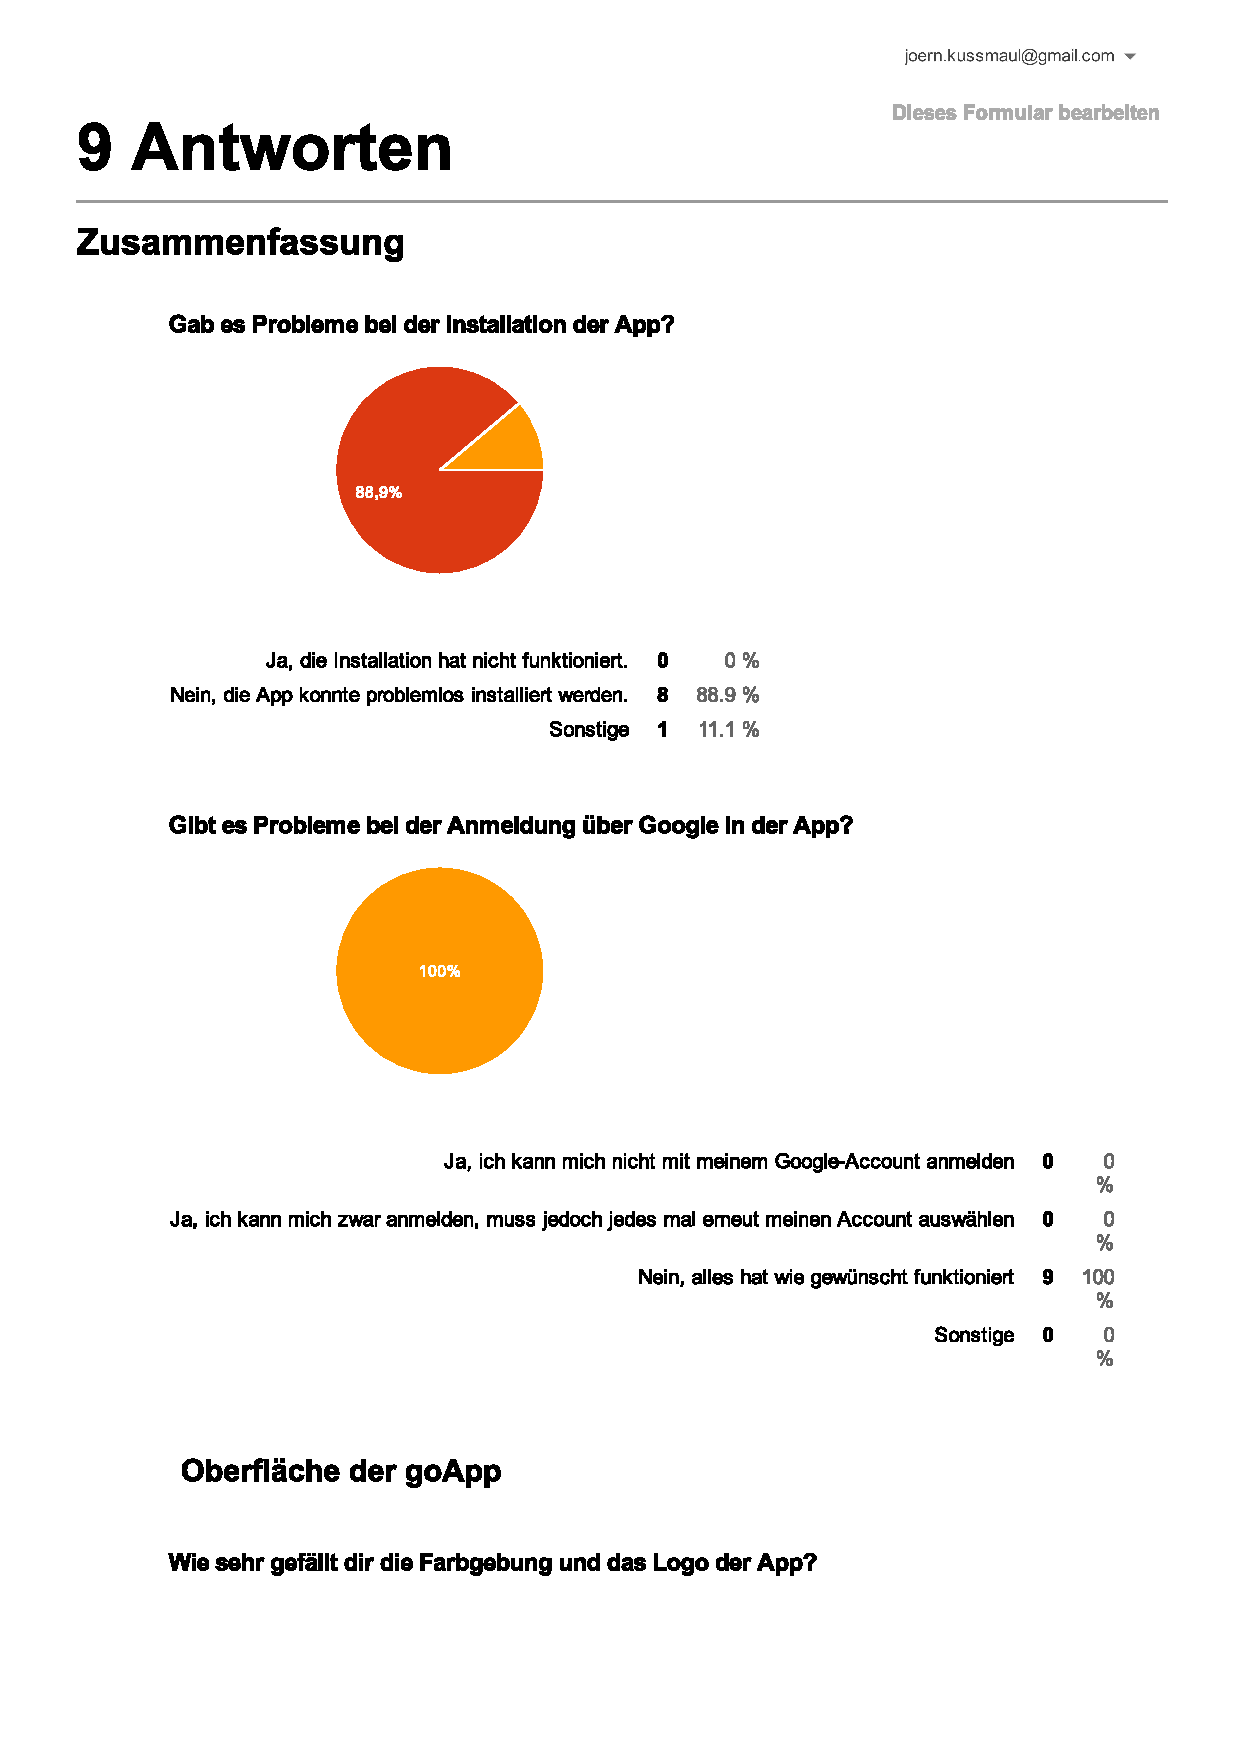
\includepdf[pages={1-5}]{UmfrageErgebnis.pdf}


\end{document}
